%++++++++++++++++++++++++++++++++++++++++
% Don't modify this section unless you know what you're doing!
\documentclass[letterpaper,12pt]{article}
\usepackage{tabularx} % extra features for tabular environment
\usepackage{amsmath}  % improve math presentation
\usepackage{graphicx} % takes care of graphic including machinery
\usepackage{pgfplots}
\pgfplotsset{width=10cm,compat=1.9}
\usepackage[margin=1in,letterpaper]{geometry} % decreases margins
\usepackage{cite} % takes care of citations
\usepackage[final]{hyperref} % adds hyper links inside the generated pdf file
\usepackage{tikz}
\usepackage{xcolor}
\usepackage{gensymb}
\usepackage{listings}
\usepackage{url}
\usepackage{tikz}
\usepackage{tzplot}
\hypersetup{
	colorlinks=true,       % false: boxed links; true: colored links
	linkcolor=blue,        % color of internal links
	citecolor=blue,        % color of links to bibliography
	filecolor=magenta,     % color of file links
	urlcolor=blue         
}
%++++++++++++++++++++++++++++++++++++++++

\begin{document}
\pagecolor{white}
\color{black}
\title{PRML - Assignment 1}
\author{Rohith Ingilela, EE19BTECH11005}
\date{\today}
\maketitle



\section{Problem Statement}
Construct a triangle, given its base, a base angle and sum
of other two sides. \\
\vspace{10pt}

Given the base BC, a base angle, say ∠B and the sum AB + AC of the other two sides of a triangle ABC, you are required to construct it.
\begin{center}
\begin{tikzpicture}
% triangle
\tzcoors(0,0)(B){$B$}[180](4,0)(C){$C$}[-45](3.5,3)(A){$A$}[45];
\tzpolygon(A){}[b](B){}[r](C){}[sloped,a](A);
% angle marks
\tzanglemark(A)(B)(C){}
\end{tikzpicture}
\end{center}

\section{Solution}

Using the cosine formula in $\triangle ABC$,
\begin{equation}
    b^2 = a^2 + c^2 - 2ac Cos B    
\end{equation}
\begin{equation}
    (b + c)(b - c) = a^2 - 2ac Cos B
\end{equation}
\begin{equation}
    or, K(b - c) = a^2 - 2ac Cos B
\end{equation}
\begin{equation}
    \text{where }  K = b + c
\end{equation}
\begin{equation}
    Kb + c (2aCosB - K) = a^2
\end{equation}

    Writing (3.4) and (3.5) into matrix form

\begin{equation}
    \begin{pmatrix}
     1 &  1 \\
     K & 2aCosB - K
    \end{pmatrix}
    \begin{pmatrix}
     b \\
     c
    \end{pmatrix}
    =
    \begin{pmatrix}
     K \\
     a^2
    \end{pmatrix}
\end{equation} \\
\vspace{10pt}
Solve matrix (3.6) for 'c' \\
\vspace{10pt}
The coordinates of $\triangle ABC$ can then be expressed as
    \begin{equation}
        \Vec{A} = c
        \begin{pmatrix}
            cos B \\
            sin B
        \end{pmatrix},
        \Vec{B} =
        \begin{pmatrix}
            0 \\
            0
        \end{pmatrix},
        \Vec{C} = 
        \begin{pmatrix}
            a \\
            0
        \end{pmatrix}
    \end{equation}
\section{Code}
\url{https://github.com/1R0H1TH/PRML/blob/main/PRML_Assignment1.py}
\section{Plot}
The above code plots Fig.\ref{fig:direction_vectors}.
\begin{figure}[!ht]
\centering
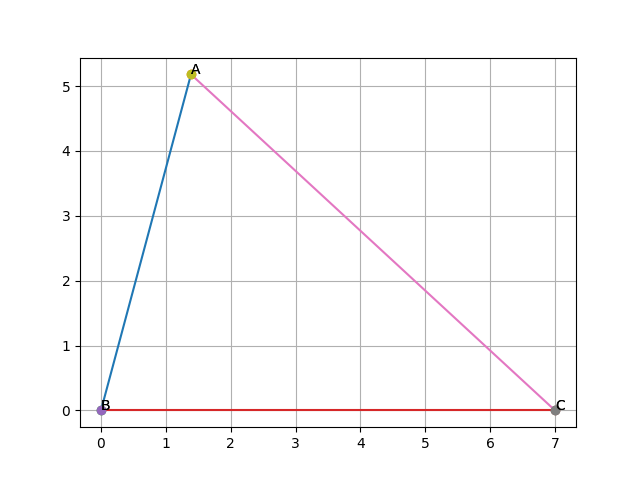
\includegraphics[width=0.75\columnwidth]{Figure_1.png}
\caption{Triangle with BC=7; $\angle$B = 75$^{\circ}$; AB + BC = 13}
\label{fig:direction_vectors}
\end{figure}

\end{document}